\subsection{Interrupts from Parallel Ports}

Parallel ports were illustrated in Figure~\ref{fig:parallel_port}, which is reproduced 
as Figure~\ref{fig:parallel_port_int}.
As the figure shows, parallel ports that support interrupts include two related registers 
at the addresses {\it Base} + 8 and {\it Base} + C.
The {\it Interruptmask} register, which has the address {\it Base} + 8, specifies whether 
or not an interrupt signal should be sent to the \GIC~when the data present at
an input port changes value.  Setting a bit location in this register to 1 allows 
interrupts to be generated, while setting the bit to 0 prevents interrupts. 
Finally, the parallel port may contain an {\it Edgecapture} register at address
{\it Base} + C.  Each bit in this register has the value 1 if the 
corresponding bit location in the parallel port has changed its value from 0 to 1.
A bit in the {\it Edgecapture} register can be cleared to 0
by writing a 1 into the corresponding bit position, which clears any associated interrupt. 

\begin{figure}[h!]
   \begin{center}
       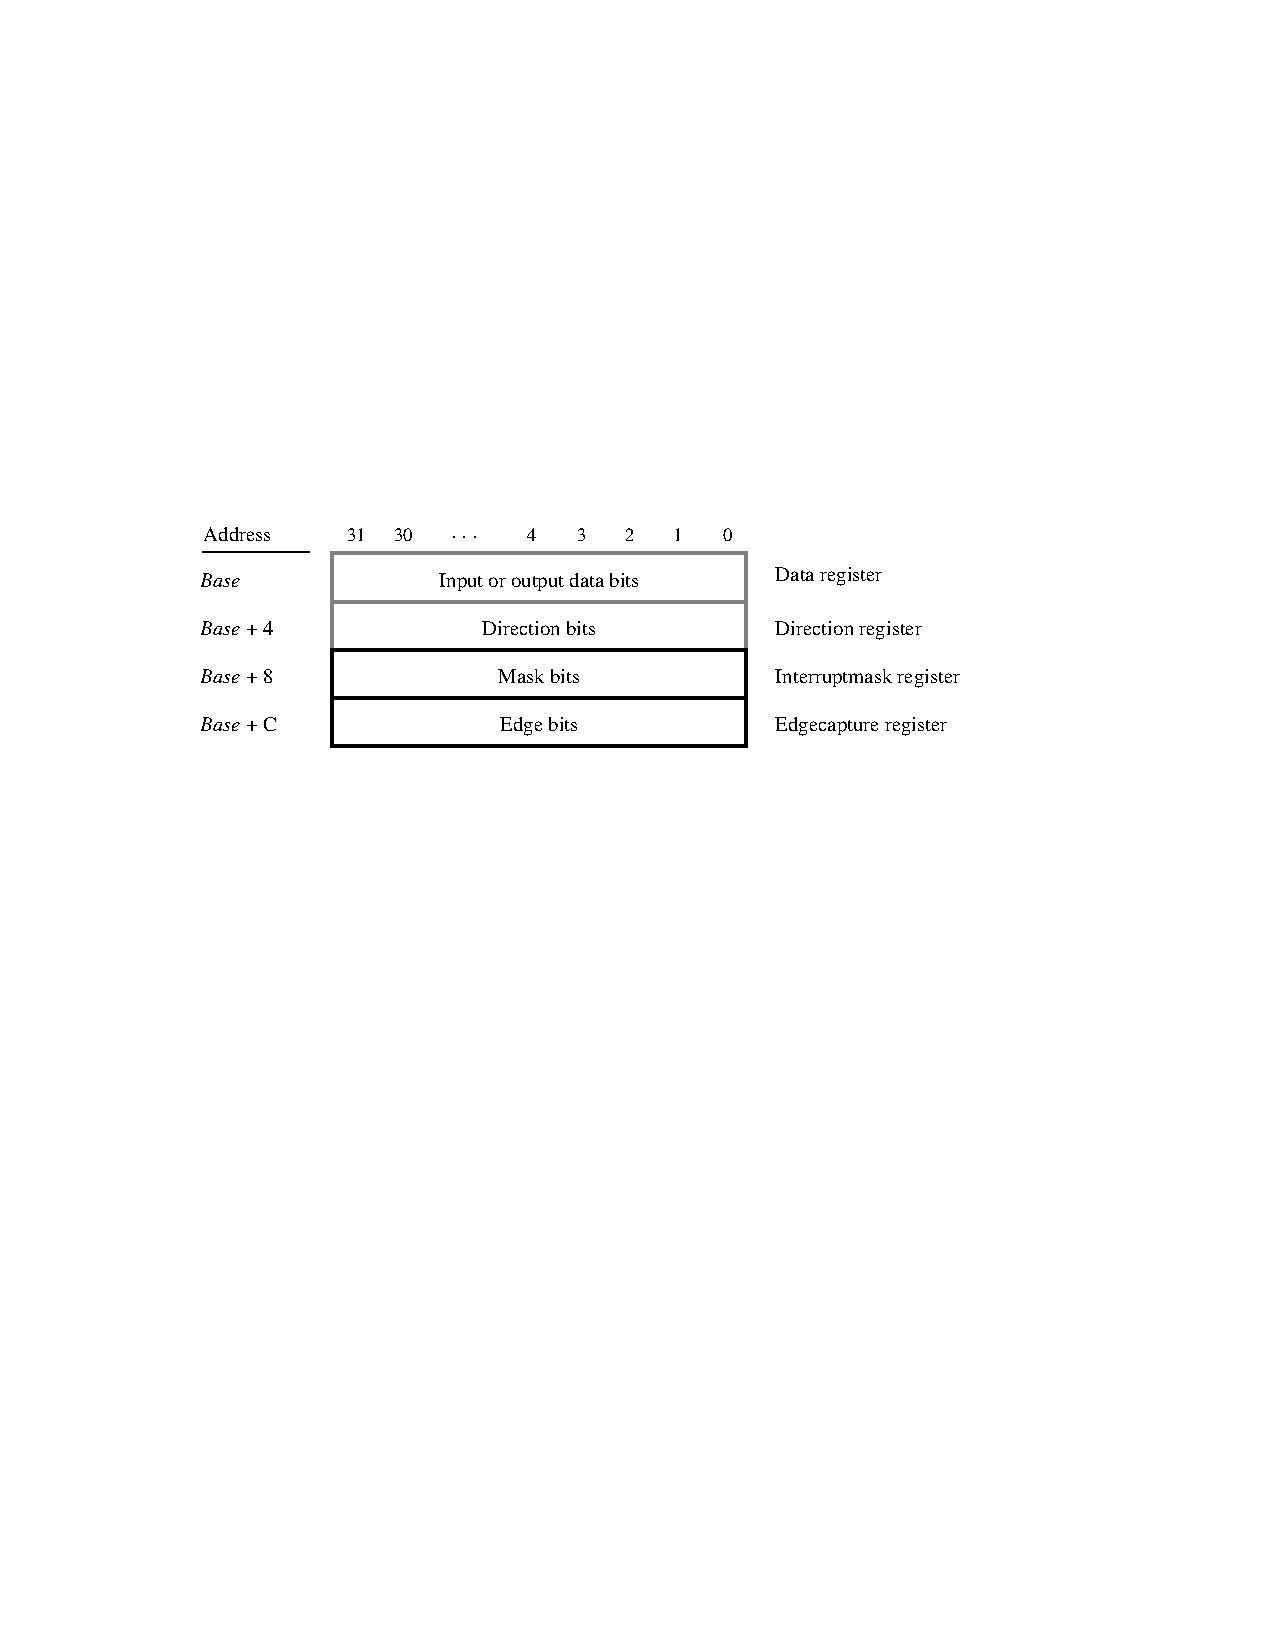
\includegraphics{../../../common/figs/Interrupts_FPGA_PP.pdf}
   \end{center}
   \caption{Registers used for interrupts from the parallel ports.}
	\label{fig:parallel_port_int}
\end{figure}


